\documentclass[10pt]{jsarticle}

\usepackage{amsmath,amsthm,amssymb}
\usepackage[dvipdfmx]{graphicx}
\usepackage{bm}
%
\usepackage{multirow}
\usepackage{wrapfig}

\usepackage{geometry}
\geometry{left=25truemm, right=25truemm, top=25truemm, bottom=25truemm}

%
\abovecaptionskip=-1pt
%\belowcaptionskip=-1pt
%
\renewcommand{\baselinestretch}{0.86} %全体の行間調整
\renewcommand{\figurename}{Fig.}
\renewcommand{\tablename}{Tab.}
%
\makeatletter 
\def\section{\@startsection {section}{1}{\z@}{1.5 ex plus 2ex minus -.2ex}{0.5 ex plus .2ex}{\large\bf}}
\def\subsection{\@startsection{subsection}{2}{\z@}{0.2\Cvs \@plus.5\Cdp \@minus.2\Cdp}{0.1\Cvs \@plus.3\Cdp}{\reset@font\normalsize\bfseries}}
\makeatother 
%

\renewcommand{\thefootnote}{\fnsymbol{footnote}}

\pagestyle{empty}

\begin{document}

%%%%%%
% はじめに
%%%%%%
\begin{center}
{\Large \textgt{MD シミュレーションによるネットワークポリマーのゴム弾性}}
\end{center}

\begin{flushright}
東亞合成 ${}^\circ$佐々木裕
\end{flushright}

\renewcommand{\thefootnote}{\fnsymbol{footnote}}
\footnote[0]{
{\bf Evaluation of Rubber Elasticity of Network Polymer by MD Simulation} \\
\underline{Hiroshi SASAKI} (Toagosei Co., Ltd. 8, Showa-Cho, Minato-ku, NAGOYA 455-0026, JAPAN)\\
Tel: +81-52-611-9923, e-mail: hiroshi\_sasaki$@$mail.toagosei.co.jp
}

\vspace{-1mm}

\section{はじめに}
%\subsection{ネットワークポリマー研究の深化と新規材料への展開}
(ネットワークポリマー研究の深化と新規材料への展開)
近年、ソフトマターの階層的な構造設計の考え方が深化し、力学特性に優れたネットワークポリマーの材料設計にも応用されている。
例えば、旧知の材料であるゴムの機能発現機構についても、フィラーとの相互作用~\cite{Igarashi2013}という観点から検討が進められ、また、脆い材料として知られているゲルも、これまでにない高強度なものが発見されてきている~\cite{Gong2010}。

これらの応用として構造材料の軽量化に繋がる新規複合材料の開発が進んでいる。
その際、一次的な力学的特性の高さだけでなく、長期使用を想定した「破壊」や「疲労」への耐久性が重要となる。
高分子材料の耐久性保証を行うためにも、力学特性の発現機構およびその劣化機構の解明が望まれている。

%\subsection{破壊にたいする粘弾性効果}
(破壊にたいする粘弾性効果)
破壊工学の考え方を端的に表せば、「系中に欠損が存在することを前提にした耐久性の評価」ということになろう。
脆性破壊する材料を想定した「Griffith 理論」での亀裂進展に伴うエネルギー開放率 $G_c$、さらには、$J$ 積分により非線形領域へ拡張された $J_c$ により破壊挙動が議論され、これらの値が靭性の指標となるとされている。
しかしながら、破断時の変形がけた違いに大きいソフトマター系の材料への適応には注意が必要である。
ゴム系材料の破壊においては粘弾性効果が報告されている。
一般に線形応答範囲で議論される時間温度換算則が大変形を伴う破壊挙動にも成立して破壊包絡線により記述できること、さらに、室温程度では伸びきりに至る前に破断する SBR がガラス転移温度に近い低温での伸長では高い伸びと強度を示すことも報告されている~\cite{Smith1969}。

粘弾性効果の影響が少ない高温、低速での破壊においては、Lake \& Thomas の指摘~\cite{Lake1967}するように、亀裂先端近傍での架橋点間のストランドの破断というモデルが成立するようであるが、実際にゴム材料を使用するような条件下においては、ゴムの破壊靭性値ははるかに大きなものとなっている。



%\subsection{力学的ヒステリシスの重要性}
(力学的ヒステリシスの重要性)
Andrews は、応力 - ひずみ関係における力学的ヒステリシスに着目し、ヒステリシスロスの存在により亀裂進展に伴うエネルギー開放量が減少し、結果として亀裂の進展が抑制されるモデルを提案している~\cite{Andrews1977}。
確かに、上述のゴムにおけるフィラーの効果~\cite{Igarashi2013}、および、DN ゲルにおける犠牲結合~\cite{Gong2010}においては大きなヒステリシスが存在し、その高靭性メカニズムはこの考え方に合致している。

これらの例はいずれも分子鎖描像より若干大きいメゾスケール領域での挙動であり、この相対的に大きなスケールでの挙動は一般に長時間緩和となる。
ヒステリシス挙動はこのスケールでしか発現しないのであろうか。
我々は、よりミクロな分子鎖描像からも、力学的ヒステリシスによる破壊耐性の向上の可能性があるのではないかと考えている。




%\subsection{疲労に対しての可逆性の重要性}
%
%一般に、破壊試験による材料の強度評価は任意の変形速度での一回の変形挙動で評価されるため、ヒステリシスの回復挙動の遅速はあまり問題にならない。
%しかしながら、材料としての耐久性を保証するためには、多様な変形速度での繰り返し変形を行う疲労試験に対する耐久性も重要である。
%この場合、適正な緩和時間で回復する可逆的なメカニズムに基づく強靭化機構が必要となる。
%
%\subsection{目指すもの}
%



%\subsection{本検討内容}
(本検討内容)
ソフトマターの構造材料への展開を標語的に言えば、「脆性破壊を伴いがちな剛直性から、設計された延性に基づく高耐久性を示す『しなやかな強さ』へのパラダイムシフト」となるであろう。
この設計された延性に必要な要件を明確にすることが本研究の目的である。

本報告では、先行研究である Everaers らの方法~\cite{Everaers1999} に従った規則構造を有するネットワークの分子動力学(MD)シミュレーションによりそのゴム弾性挙動の変形速度依存性と緩和時間との関連について検討を行い、時間温度換算則が成り立つような線形粘弾性の枠組みでのヒステリシスを考察した。


\section{シミュレーション}

Everaers らの方法~\cite{Everaers1999}に従い、ストランド長を規定した規則構造を有する ``Network Model'' を作成し、その平衡状態および一軸伸長時の振る舞いについて、OCTA 上の COGNAC シミュレーターを用いた分子動力学シミュレーションにより評価した。
なお、ストランドには、Kremer らが提唱した「鎖のすり抜け」を抑制し絡み合いを表した ''KG Polymer'' と呼ばれるビーズ・スプリングモデル~\cite{Kremer1990} を用いた。

\subsection{ポテンシャルの設定}

非結合ポテンシャルとして各ビーズ間に LJ ポテンシャル $U_{LJ}(r)$、ボンドポテンシャルには伸びきり効果の入った FENE-LJ ポテンシャル $U_{FENE}(r)$ を用い、パラメタは一般的な $\epsilon = \sigma = 1, R = 1.5, K=30$ とした。

\newpage


\begin{wrapfigure}{r}{65mm}
\vspace{-1\baselineskip}
	\begin{center}
	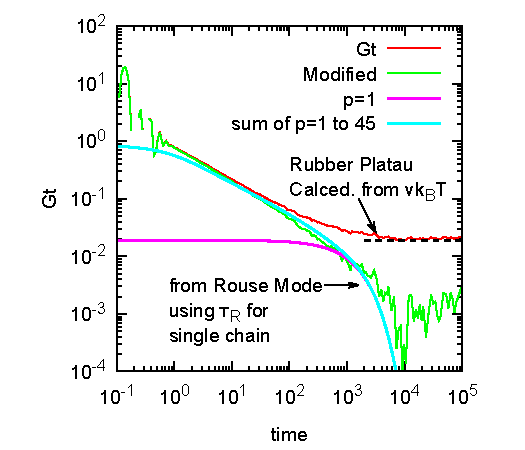
\includegraphics[width=60mm]{./fig/Gt_loglog.pdf}
	\caption{Stress Relaxation Curve calcd. by Green-Kubo formula}
	\label{fig: Relux}
	\end{center}
\vspace{5mm}
\end{wrapfigure}

\subsection{ネットワークモデル}
44 個のビーズからなるストランドが結節点において 4 本結合しダイヤモンド構造となるようにユニットセル中に配置した。
その際、ストランドの末端間距離をメルトと同一としたうえで、一般的な ''KG Polymer'' と同様の密度($\rho = 0.85$)となるように、複数のネットワークが相互貫入した IPN 構造の多重度(Multi = 9)を決めた。

\begin{wrapfigure}{r}{65mm}
\vspace{-3\baselineskip}
	\begin{center}
	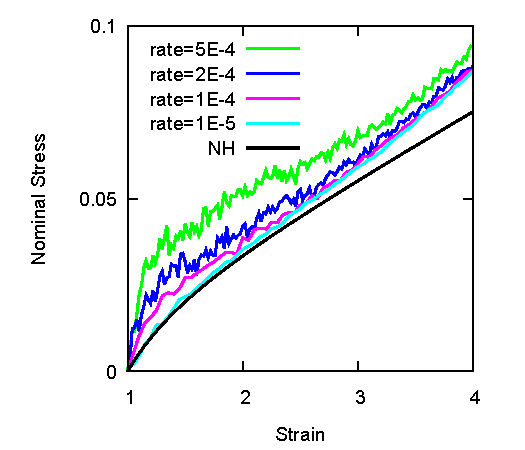
\includegraphics[width=60mm]{./fig/N44_SS_mid.pdf}
	\caption{Uniaxial Elongation SS Curves for different stretching rate}
	\label{fig: stretch}
	\end{center}
\vspace{-5mm}
\end{wrapfigure}

\section{結果と考察}
\subsection{ネットワークの線形粘弾性}

平衡状態の MD シミュレーションから Green-Kubo 公式により求めたネットワークの応力緩和関数(赤線)および $\nu k_B T$ から算出したゴム弾性プラトーの値を緩和関数から差し引いたもの(緑線)を併せて Fig.\ref{fig: Relux} に示した。
また、ストランドと同等な自由鎖(N=46)のラウス緩和(最長ラウス緩和時間 $\tau_R = 2700$)についても示している。

この類似性から、少なくとも、今回検討した単純な規則構造を有するネットワークにおいては、架橋構造の緩和時間への寄与は少ないものと推定できた。

\begin{wrapfigure}{r}{65mm}
%\vspace{-1\baselineskip}
	\begin{center}
	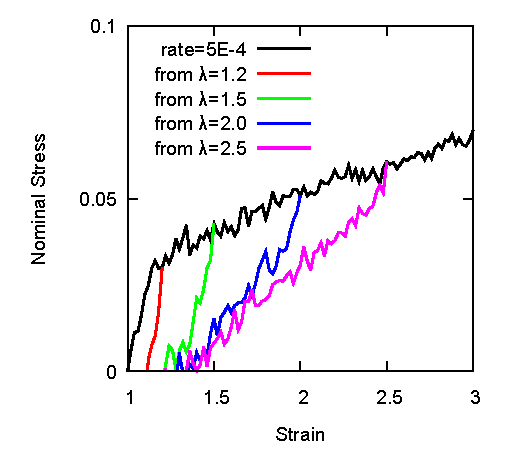
\includegraphics[width=60mm]{./fig/N44_rev_SS.pdf}
	\caption{Hysteresis Curves from different elongation position}
	\label{fig: hyst}
	\end{center}
\vspace{-5mm}
\end{wrapfigure}

\subsection{一軸伸長}
変形速度の異なる一軸伸長($5 \times 10^{-4} \sim 1 \times 10^{-5} \lambda/\tau$)時の SS カーブを、ネオフッキアンモデルと共に、Fig. \ref{fig: stretch} に示した。
伸長速度の低減により、$\lambda<2$ 程度の小さなひずみではネオフッキアンモデルに合致した。
また、任意の変形量でのステップ変形からの応力緩和を調べたところ、その最長緩和時間が自由鎖の
 $\tau_R$ と同程度であることを確認した。


\subsection{力学的ヒステリシス}

最長緩和時間の逆数程度のオーダーである変形速度($5E^{-4}\lambda/\tau$)での一軸伸長において、任意の変形量($\lambda = 1.2, 1.5, 2.0, 2.5$)まで伸長した後に同等の変形速度で圧縮を行い、力学的ヒステリシスを測定した結果を、Fig. \ref{fig: hyst} に示した。
また、伸長速度を遅くすることにより、ヒステリシス強度が減少することも確認できた。
\section{おわりに}

本報告においては、単純な規則構造を有するネットワークの線形緩和現象と任意の変形速度での力学応答との関係から力学的ヒステリシスが生じることを確認し、その発現メカニズムがストランドの緩和現象に起因するものであることを推定した。
実際の破壊現象はこれほど単純ではなく、大変形時の非線形応答を考慮する必要は大きいと考えている。
さらなる検討を進めていきたい。

\bibliographystyle{../achemso}
\bibliography{D:/Dropbox/Bibliography/library.bib}


\end{document}